% Schwingung, gedämpft (RLC-Serienschwingkreis mit u über C)
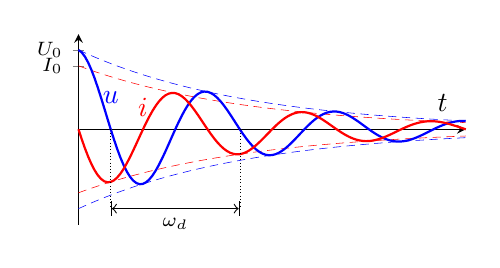
\begin{tikzpicture}[x=1mm,y=1mm] % gilt für tikz-coordinaten außerhalb der axis-environment
    \draw[draw=none] (-6,-2) rectangle (50,25); % Bildrahmen, Koordinatenbezug auf (0,0) des \begin{axis}...\end{axis} pgfplots, für
    \begin{axis}[
        axis lines=center,
        xlabel={$t$},
        x label style={xshift=-3pt,yshift=3pt},
        xmin=0, xmax=3,% 3 wt
        ymin=-1.5, ymax=1.5,
        xtick={\empty},
        xticklabel={\empty},
        xminorticks=false,
        ytick={+1,+1.25},
        yticklabels={$\scriptstyle{I_{0}}$,$\scriptstyle{U_{0}}$},
        yminorticks=false,
        domain=0:3,
        samples=121,
        grid=none,
        width=6.5cm,
        height=4.0cm,
        clip=false,
    ]
        \addplot+[mark=none,very thin,blue,densely dashed,] {1.25 * +e^(-x*0.75)};
        \addplot+[mark=none,very thin,blue,densely dashed,] {1.25 * -e^(-x*0.75)};
        \addplot+[mark=none,very thin,red,densely dashed,]  {1.0 * +e^(-x*0.75)};
        \addplot+[mark=none,very thin,red,densely dashed,]  {1.0 * -e^(-x*0.75)};

        \addplot+[mark=none,thick,blue,solid,]   {1.25*sin(x*360+90) * e^(-x*0.75)};    % u plot
        \addplot+[mark=none,thick,red,solid,]    {-1.0*sin(x*360) * e^(-x*0.75)};        % i plot
        
        \node[blue] at (axis cs:0.25,0.5) {$u$};
        \node[red] at (axis cs:0.50,0.35) {$i$};

        \addplot+[mark=none,very thin,black,densely dotted,] coordinates {(0.25,-0.0)(0.25,-1.25)};
        \addplot+[mark=none,very thin,black,densely dotted,] coordinates {(1.25,-0.0)(1.25,-1.25)};
        \addplot+[mark=none,black,solid,|<->|] coordinates {(0.25,-1.25)(1.25,-1.25)} node[midway,below] {$\scriptstyle{\omega_d}$};% T0=2pi/w0 $\scriptstyle{2\pi/\omega_0}$
    \end{axis}
\end{tikzpicture}%